% Responsable: A
\section{Análisis exploratorio}

\subsection{Fuente y recolección de los datos}
Los datos provienen de la base \emph{Maternal Health Risk} del repositorio UCI
Machine Learning Repository \citep{ahmed2020maternal}, disponible en
\url{https://archive.ics.uci.edu/dataset/863/maternal+health+risk}. Los registros
se recolectaron en hospitales, clínicas comunitarias y centros de atención
materna de zonas rurales de Bangladesh mediante un sistema de monitoreo de riesgo
basado en sensores IoT. La base tiene 1.014 registros y no incluye un
identificador por paciente, por lo que cada fila se trata como un registro de
medición y no necesariamente como una gestante distinta.

\subsection{Variables}
La base contiene seis variables predictoras continuas y la variable objetivo
(Tabla~\ref{tab:variables}). No hay datos faltantes en ninguna variable.

\begin{table}[h]
\centering
\caption{Variables de la base.}
\label{tab:variables}
\small
\begin{tabular}{lll}
\toprule
Variable & Descripción & Unidad\\
\midrule
Age         & Edad de la gestante          & años\\
SystolicBP  & Presión arterial sistólica   & mm Hg\\
DiastolicBP & Presión arterial diastólica  & mm Hg\\
BS          & Glucosa en sangre            & mmol/L\\
BodyTemp    & Temperatura corporal         & °F\\
HeartRate   & Frecuencia cardíaca          & lpm\\
RiskLevel   & Nivel de riesgo (bajo, medio, alto) & ordinal\\
\bottomrule
\end{tabular}
\end{table}

\subsection{Estadísticas descriptivas}
La Tabla~\ref{tab:descriptivas} resume la base inicial. Se destacan cuatro
hallazgos. La frecuencia cardíaca tiene un mínimo de 7 lpm, un valor
biológicamente imposible que corresponde a un error de registro. La glucosa
tiene una distribución sesgada a la derecha: el 75\,\% de los registros está por
debajo de 8,0 mmol/L, pero hay valores de hasta 19 mmol/L, propios de una
hiperglucemia severa. Algunas variables están muy concentradas en valores
redondos, probablemente por el redondeo de los equipos: 804 registros tienen una
temperatura de exactamente 98\,°F y 449 una presión sistólica de 120 mm Hg, lo
que reduce la variabilidad que estas variables pueden aportar al modelo.
Finalmente, la edad va de 10 a 70 años; los extremos son poco probables en un
estudio de salud materna, pero no imposibles, por lo que se conservan.

\begin{table}[h]
\centering
\caption{Estadísticas descriptivas de la base inicial ($N=1.014$).}
\label{tab:descriptivas}
\small
\setlength{\tabcolsep}{3.5pt}
\begin{tabular}{lrrrrrr}
\toprule
 & Age & Sys & Dia & BS & Temp & HR\\
\midrule
Media    & 29.87 & 113.20 & 76.46 & 8.73 & 98.67 & 74.30\\
Desv.    & 13.47 & 18.40 & 13.89 & 3.29 & 1.37 & 8.09\\
Mínimo   & 10 & 70 & 49 & 6.0 & 98.0 & 7\\
Q1       & 19 & 100 & 65 & 6.9 & 98.0 & 70\\
Mediana  & 26 & 120 & 80 & 7.5 & 98.0 & 76\\
Q3       & 39 & 120 & 90 & 8.0 & 98.0 & 80\\
Máximo   & 70 & 160 & 100 & 19.0 & 103.0 & 90\\
\bottomrule
\end{tabular}
\end{table}

\subsection{Procesamiento}
La auditoría de calidad mostró que 562 filas son copias exactas de otra, de modo
que solo hay 452 registros únicos. Como la base no permite saber si las copias
son tomas de la misma gestante, tratarlas como observaciones independientes
haría que la posterior pareciera más precisa de lo que es y facilitaría la fuga
de información entre entrenamiento y prueba. Por esto se trabaja con los
registros únicos, y la base completa se usa solo como análisis de sensibilidad.
Se conservaron los 35 perfiles que tienen los mismos signos vitales y una
etiqueta distinta, ya que reflejan que la etiqueta depende de información que no
está en la base. Además, se eliminó el registro con frecuencia cardíaca de 7 lpm,
con lo que la base principal queda con 451 registros.

El nivel de riesgo se codificó como variable ordinal (bajo $=0$, medio $=1$,
alto $=2$). La partición en entrenamiento (75\,\%) y prueba (25\,\%) se hizo sobre
los perfiles únicos de signos vitales, estratificando por nivel de riesgo, para
que un mismo perfil no quedara en ambos conjuntos; así se obtuvieron 334
registros de entrenamiento y 117 de prueba. Las variables se estandarizaron con
la media y la desviación estándar del conjunto de entrenamiento.

\subsection{Gráficas}
Eliminar los duplicados cambia la distribución de las clases
(Figura~\ref{fig:clases}): el riesgo bajo pasa de 40,0\,\% a 51,8\,\% y el riesgo medio,
que es la clase con más repeticiones, baja de 33,1\,\% a 23,5\,\%. En la base
principal las clases no están balanceadas, lo que se tiene en cuenta al
estratificar la partición y al elegir las métricas de evaluación.

\begin{figure}[h]
\centering
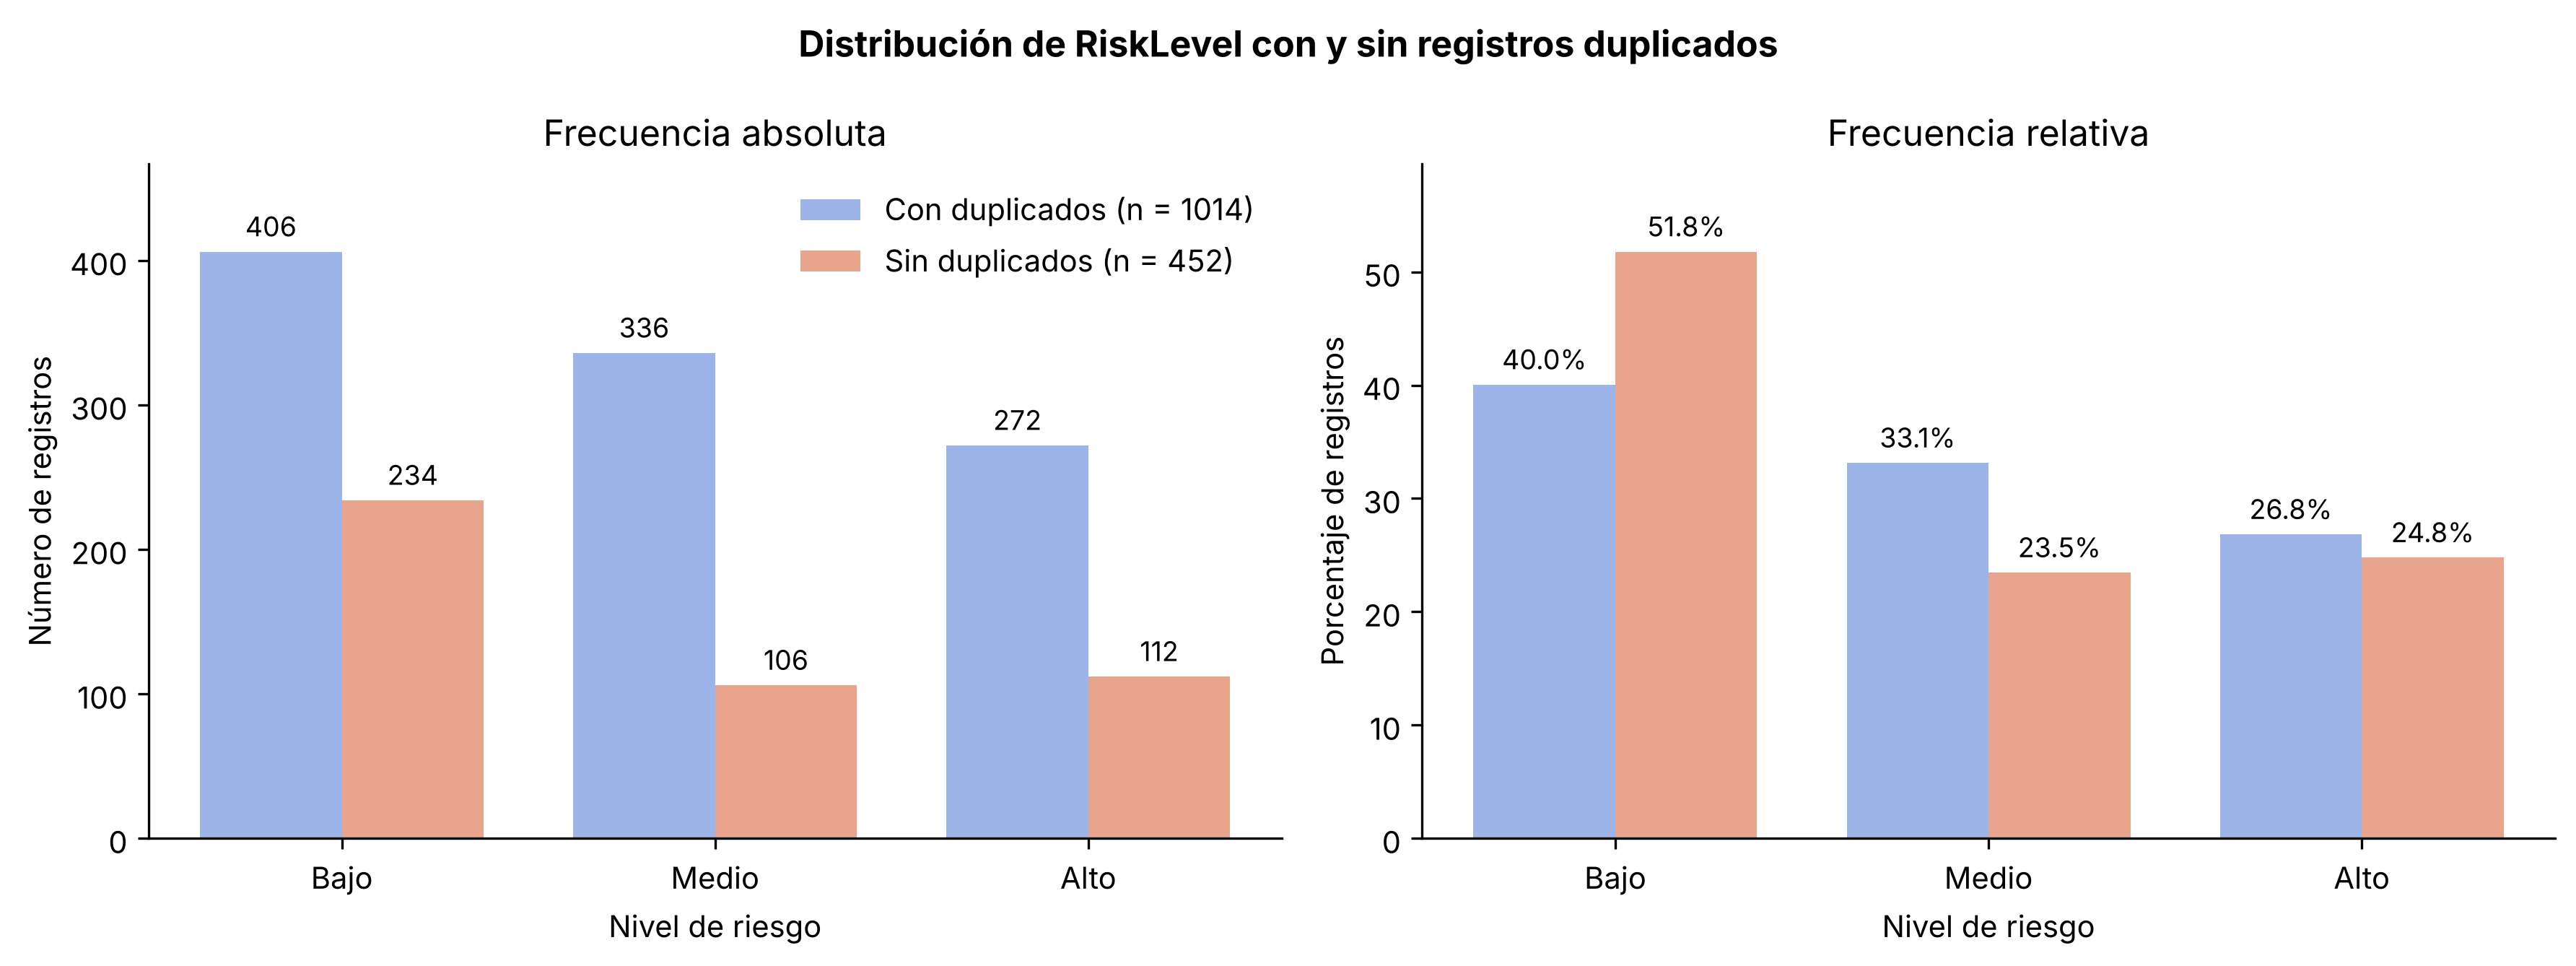
\includegraphics[width=\columnwidth]{eda_clases_duplicados.png}
\caption{Distribución del nivel de riesgo con y sin registros duplicados.}
\label{fig:clases}
\end{figure}

En la base inicial, la mayoría de las variables tienen una distribución unimodal
con colas largas hacia los valores altos, propias de los casos clínicos severos
(Figura~\ref{fig:histogramas}).

\begin{figure*}[t]
\centering
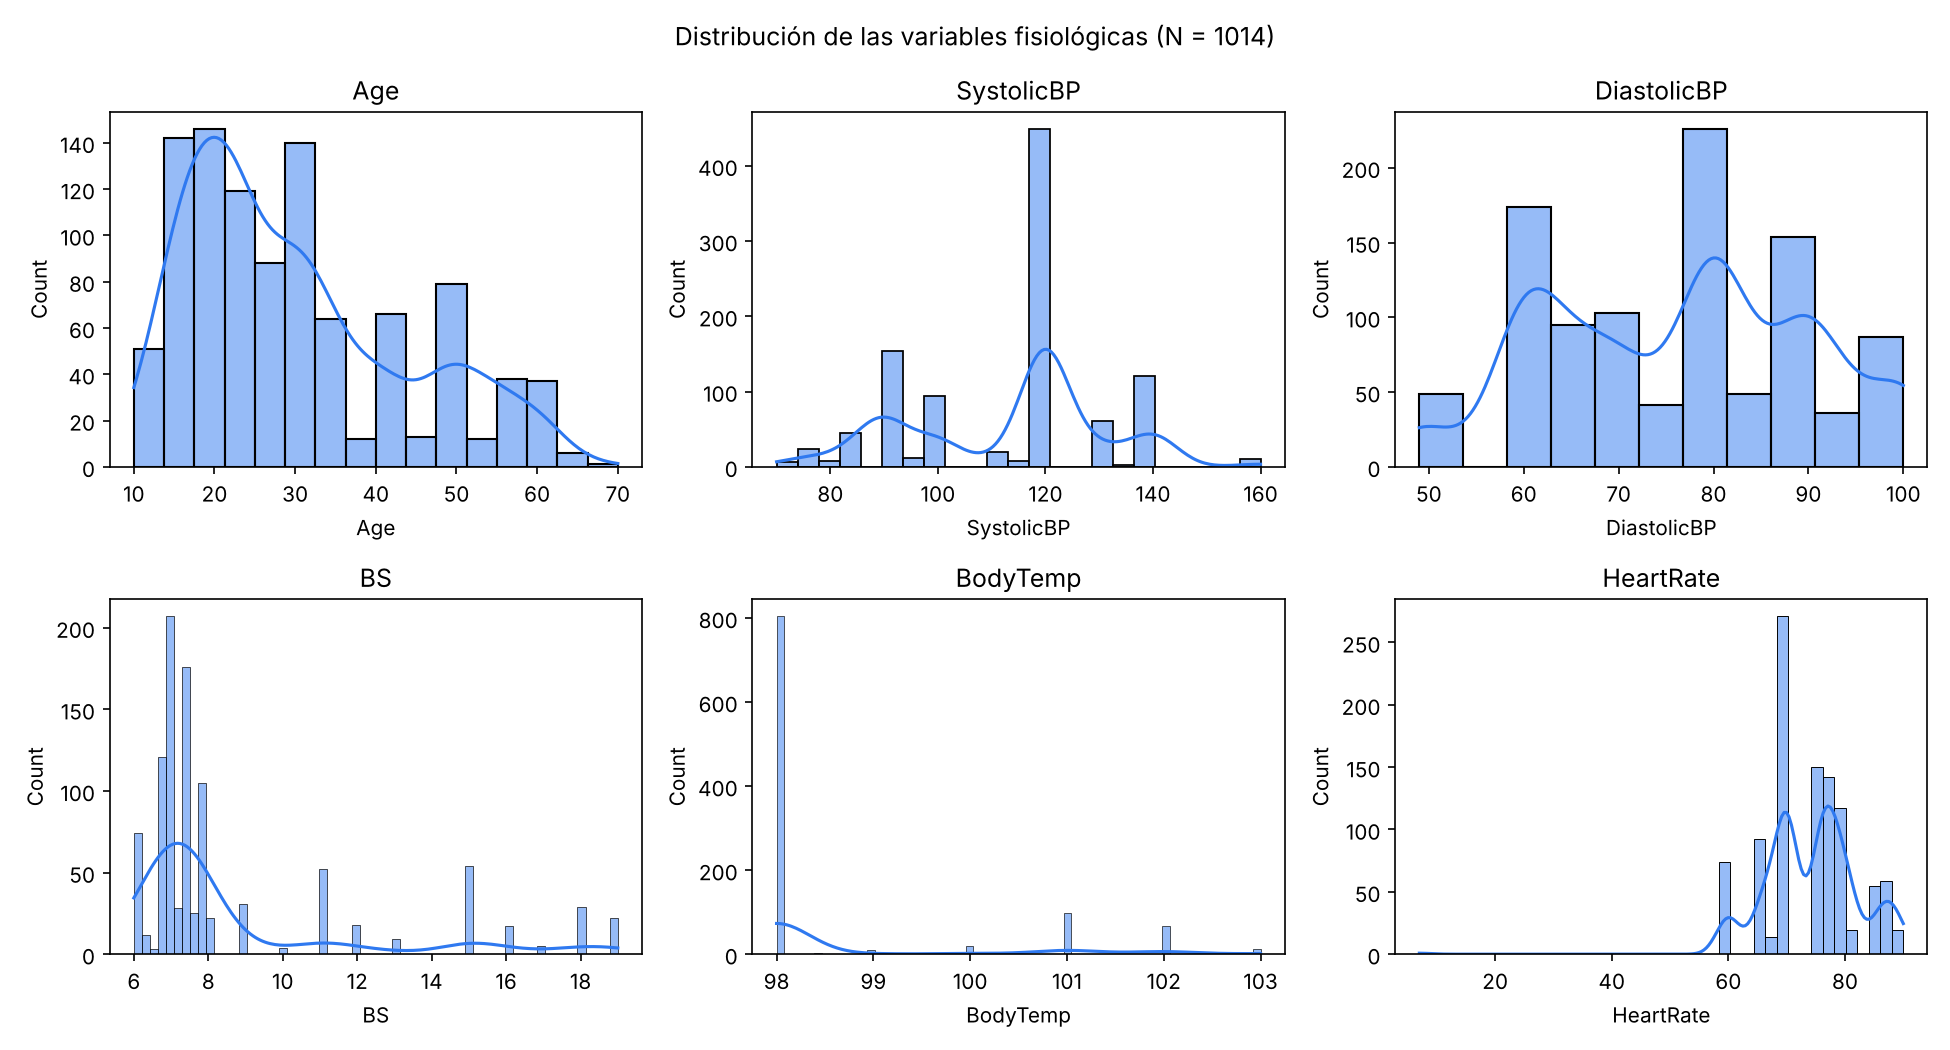
\includegraphics[width=0.85\textwidth]{eda_histogramas_con_duplicados.png}
\caption{Distribución de las variables fisiológicas en la base inicial ($N=1.014$).}
\label{fig:histogramas}
\end{figure*}

La comparación por nivel de riesgo con los registros únicos
(Figura~\ref{fig:boxplots}) muestra que las tres clases se solapan en todas las
variables. La clase de riesgo alto es la más fácil de distinguir, sobre todo por
la glucosa (mediana de 11,0 mmol/L frente a 7,2 y 7,0 en riesgo bajo y medio) y por
la edad (33,5 años frente a 22 y 25,5). Las clases de riesgo bajo y medio son las
más difíciles de separar.

\begin{figure*}[t]
\centering
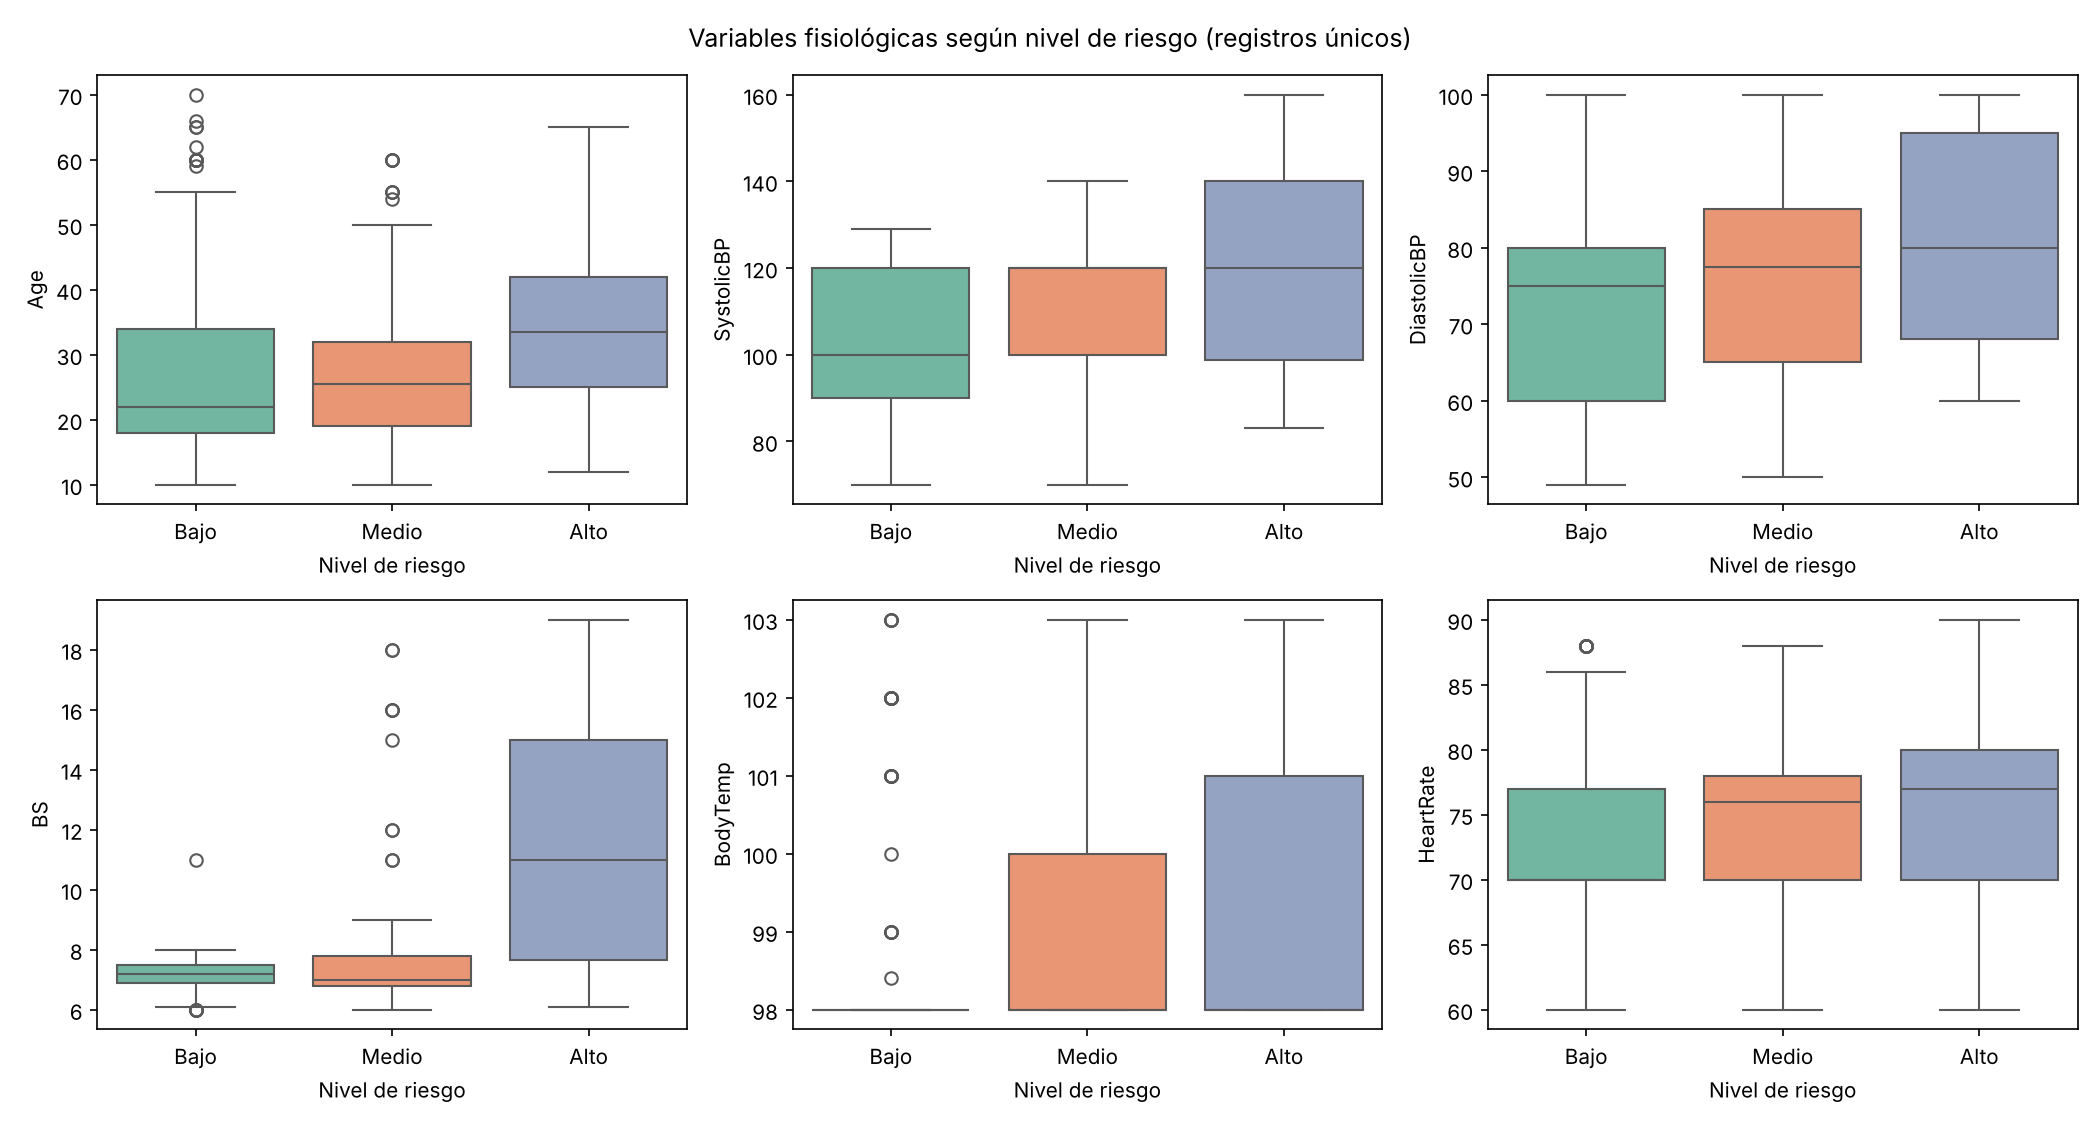
\includegraphics[width=0.85\textwidth]{eda_boxplots_por_riesgo_sin_duplicados.png}
\caption{Variables fisiológicas según el nivel de riesgo (registros únicos, $n=451$).}
\label{fig:boxplots}
\end{figure*}

En la matriz de correlación de la base inicial (Figura~\ref{fig:correlaciones}),
la glucosa es la variable más asociada con el nivel de riesgo ($r=0.57$), seguida
de la presión sistólica ($0.40$) y la diastólica ($0.35$); la temperatura ($0.16$) y
la frecuencia cardíaca ($0.19$) tienen asociaciones bajas. Las dos presiones están
muy correlacionadas entre sí ($r=0.79$), lo que puede dificultar separar sus
efectos en el modelo. Con los registros únicos la glucosa sigue siendo la variable
más asociada ($0.55$), pero las correlaciones de la presión diastólica ($0.25$) y
la edad ($0.18$) bajan, lo que indica que las repeticiones inflaban su aparente
relación con el riesgo.

\begin{figure*}[t]
\centering
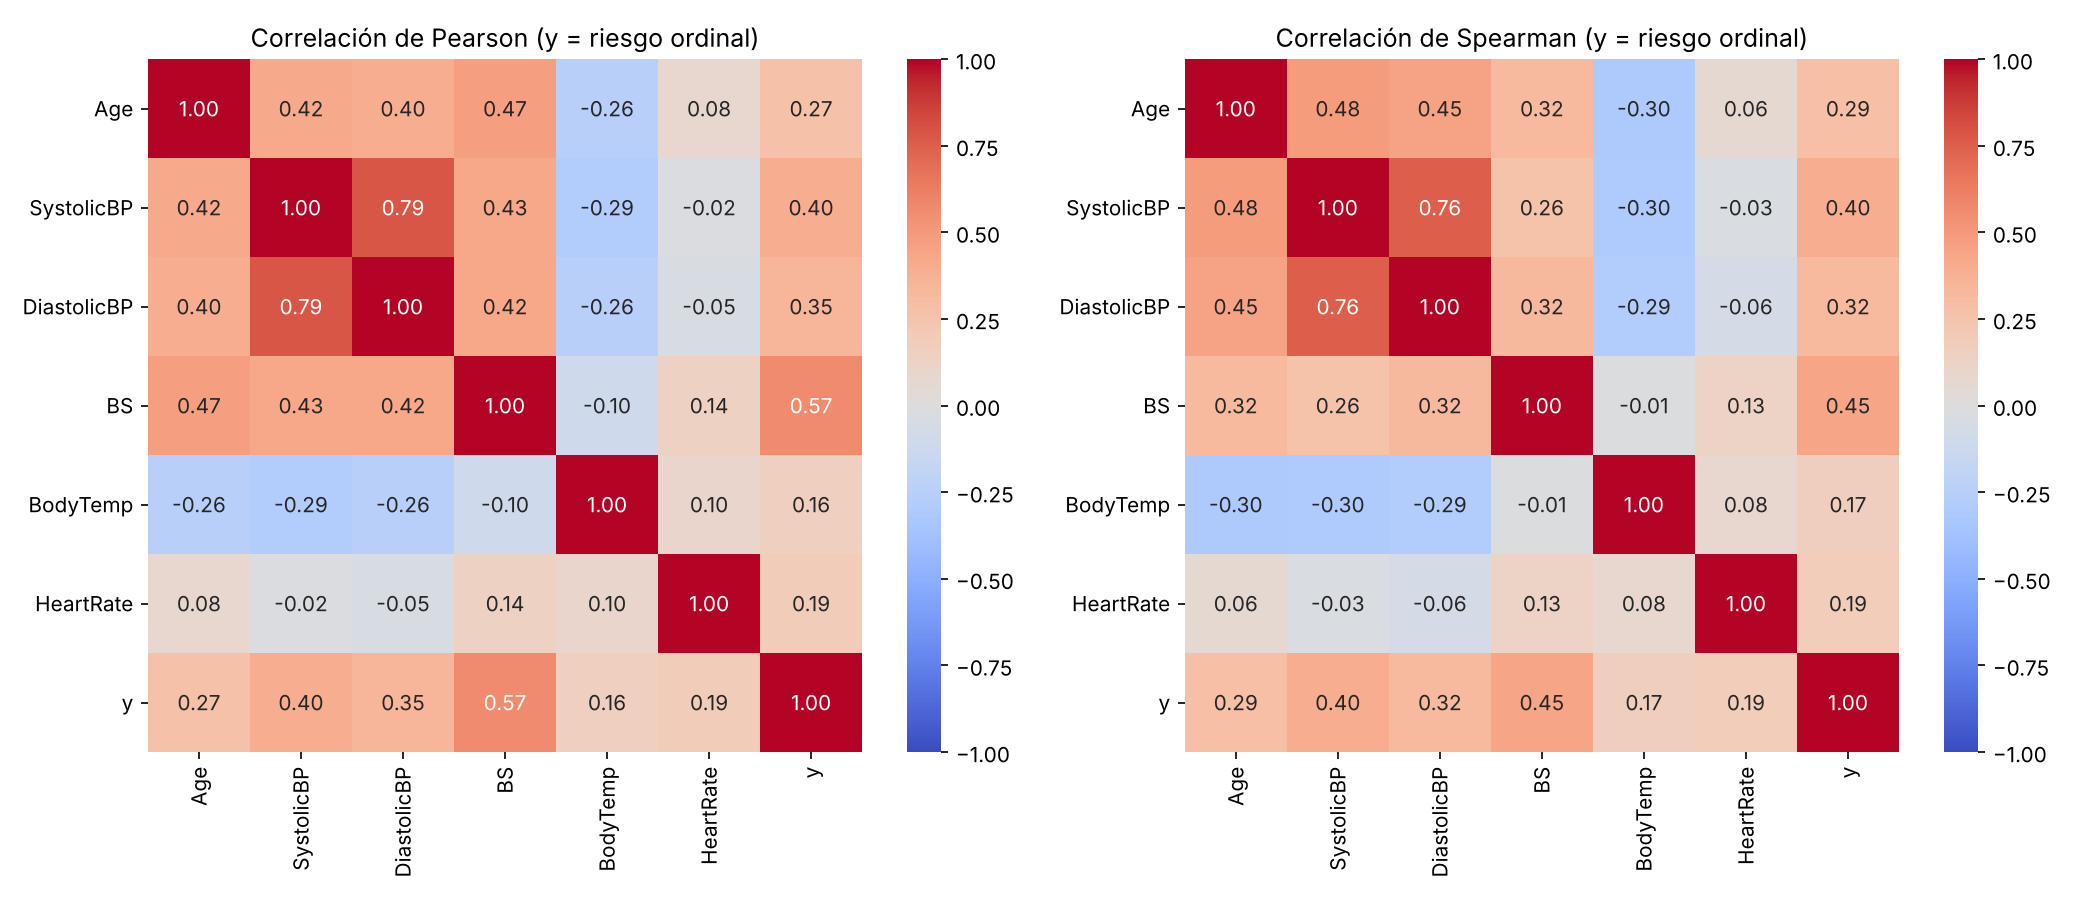
\includegraphics[width=0.85\textwidth]{eda_correlaciones_con_duplicados.png}
\caption{Correlaciones de Pearson y Spearman entre las variables y el nivel de riesgo (base inicial).}
\label{fig:correlaciones}
\end{figure*}
